\documentclass[aspectratio=169]{beamer} % Widescreen for modern look

% --- Theme & Styling ---
\usetheme{Warsaw}       
\usecolortheme{seahorse} 
\useoutertheme{shadow}  

% --- Packages ---
\usepackage{xcolor}
\usepackage{booktabs}
\usepackage{tikz}
\usepackage{amssymb} % Required for checkmarks
\usepackage{caption}

% --- FIXED: Added 'shapes.symbols' for the CPU Cloud diagram ---
\usetikzlibrary{shapes.geometric, shapes.symbols, arrows, positioning, shadows.blur, trees, calc}

% --- Custom Colors ---
\definecolor{DeepBlue}{RGB}{0, 50, 100}
\definecolor{TechOrange}{RGB}{255, 140, 0}

% --- Setup Title ---
\title[RPN Calculator Project]{ RPN Calculator}
\subtitle{Advanced Stack Algorithms \& GUI Design}

% --- FIXED: Clean metadata in [] (no \\) to stop PDF warnings ---
\author[Ramsh and Suresh Kumar]{
	\textbf{Gautam Ramsh} \\ 
	\textbf{Subash Karapparambu Suresh Kumar}
}
\institute{Computer Science}
\date{\today}

\begin{document}
	
	% ==========================================
	% PART 1: INTRO (Slides 1-3)
	% ==========================================
	
	% Slide 1: Title
	\begin{frame}
		\titlepage
	\end{frame}
	
	% Slide 2: Agenda
\begin{frame}{Project Roadmap}
	% This lists all sections (1-5) in a single vertical column
	\tableofcontents
\end{frame}
	
	% Slide 3: The Core Concept
	% FIXED: Escaped & symbol
	\section{Context \& Theory}
	\begin{frame}{What is Reverse Polish Notation?}
		\begin{block}{Definition}
			\textbf{RPN (Postfix Notation)} is a mathematical syntax where operators \textbf{follow} their operands.
		\end{block}
		
		\vspace{1cm}
		\centering
		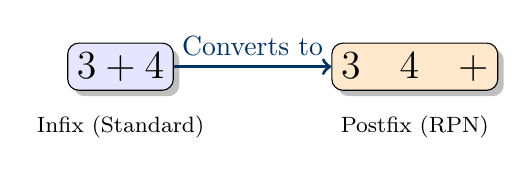
\begin{tikzpicture}[node distance=2cm]
			\node[draw, fill=blue!10, rounded corners, drop shadow] (infix) {\Large $3 + 4$};
			\node[draw, fill=TechOrange!20, rounded corners, drop shadow, right=of infix] (postfix) {\Large $3 \quad 4 \quad +$};
			
			\draw[->, very thick, DeepBlue] (infix) -- node[above] {Converts to} (postfix);
			
			\node[below=0.2cm of infix, font=\footnotesize] {Infix (Standard)};
			\node[below=0.2cm of postfix, font=\footnotesize] {Postfix (RPN)};
		\end{tikzpicture}
	\end{frame}
	
	% ==========================================
	% PART 2: HISTORY (Slides 4-6)
	% ==========================================
	
	% Slide 4: The Infix Problem
	\begin{frame}{The Problem with Standard Math (Infix)}
		Why did engineers reinvent math notation?
		\vspace{0.5cm}
		\begin{enumerate}
			\item \textbf{Ambiguity:} $3 + 4 \times 5$
			\item \textbf{Parentheses Hell:} $((3+4) \times (5-2)) / 6$
			\item \textbf{Memory Heavy:} Computers need complex recursion to solve Infix.
		\end{enumerate}
		
		\vspace{0.5cm}
		\begin{alertblock}{The Computer's Struggle}
			Standard math forces computers to scan back and forth to find priority (PEMDAS).
		\end{alertblock}
	\end{frame}
	
	% Slide 5: The HP Solution
	\begin{frame}{The Hewlett-Packard Revolution (1972)}
		\begin{columns}
			\column{0.6\textwidth}
			In 1972, the \textbf{HP-35} changed everything.
			\begin{itemize}
				\item It was the first handheld scientific calculator.
				\item It had \textbf{No Equals Key (=)}.
				\item It had \textbf{No Parentheses Keys ( )}.
			\end{itemize}
			\vspace{0.5cm}
			\textbf{Result:} It was faster and used less battery/memory than any competitor.
			
			\column{0.4\textwidth}
			\centering
			% Placeholder for HP-35 Image
			\begin{tikzpicture}
				\node[draw, fill=gray!20, minimum width=3cm, minimum height=4cm, align=center] {
					\includegraphics[width=0.5\textwidth]{hp35.jpg}
				
				};
			\end{tikzpicture}
			\captionof{figure}{\footnotesize The HP-35}
		\end{columns}
	\end{frame}
	
	% Slide 6: Visualizing the Tree
	\begin{frame}{Visualizing the Logic: Expression Trees}
		Expression: \textbf{$(3 + 4) \times 5$}
		\vspace{0.5cm}
		\centering
		
		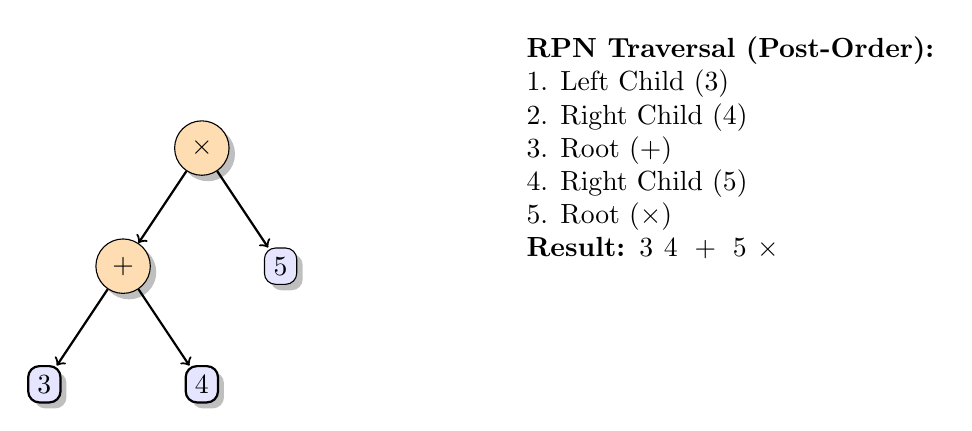
\begin{tikzpicture}[level distance=1.5cm, sibling distance=2cm, 
			edge from parent/.style={draw, thick, ->},
			op/.style={circle, draw, fill=TechOrange!30, drop shadow},
			num/.style={rectangle, draw, fill=blue!10, drop shadow, rounded corners}]
			
			\node[op] {$\times$}
			child { node[op] {$+$}
				child { node[num] {3} }
				child { node[num] {4} }
			}
			child { node[num] {5} };
			
			\node[right=4cm, align=left] {
				\textbf{RPN Traversal (Post-Order):}\\
				1. Left Child (3)\\
				2. Right Child (4)\\
				3. Root (+)\\
				4. Right Child (5)\\
				5. Root ($\times$)\\
				\textbf{Result: $3 \ 4 \ + \ 5 \ \times$}
			};
		\end{tikzpicture}
	\end{frame}
	
	
	% ==========================================
	% PART 3: MECHANICS (Slides 7-13)
	% ==========================================
	% FIXED: Escaped & symbol
	\section{Mechanics \& Algorithms}
	
	% Slide 7: The Stack Theory
	\begin{frame}{The Data Structure: Stack (LIFO)}
		The engine of RPN is the \textbf{Stack}.
		\begin{itemize}
			\item \textbf{LIFO:} Last-In, First-Out.
			\item Think of a stack of plates.
		\end{itemize}
		\vspace{0.5cm}
		\centering
		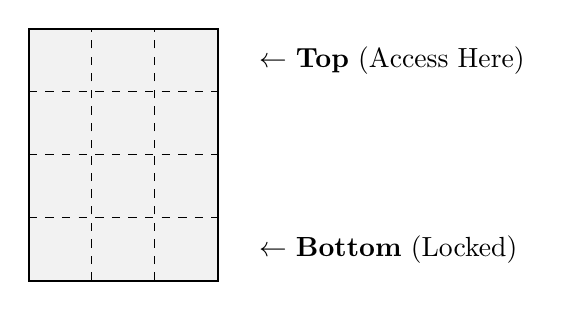
\begin{tikzpicture}[scale=0.8]
			% Stack Container
			\draw[thick, fill=gray!10] (0,0) -- (0,4) -- (3,4) -- (3,0) -- cycle;
			\draw[dashed] (0,0) grid (3,4);
			
			% Annotations
			\node[anchor=west] at (3.5, 3.5) {$\leftarrow$ \textbf{Top} (Access Here)};
			\node[anchor=west] at (3.5, 0.5) {$\leftarrow$ \textbf{Bottom} (Locked)};
		\end{tikzpicture}
	\end{frame}
	
	% Slide 8: Operation PUSH
	\begin{frame}{Core Operation 1: PUSH}
		\textbf{PUSH:} Adds a value to the top of the stack.
		\vspace{1cm}
		\centering
		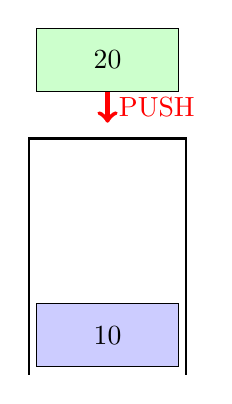
\begin{tikzpicture}
			% Stack
			\draw[thick] (0,0) -- (0,3) -- (2,3) -- (2,0);
			\node[draw, fill=blue!20, minimum width=1.8cm, minimum height=0.8cm] at (1, 0.5) {10};
			
			% Incoming
			\node[draw, fill=green!20, minimum width=1.8cm, minimum height=0.8cm] (new) at (1, 4) {20};
			\draw[->, ultra thick, red] (new) -- (1, 3.2) node[midway, right] {PUSH};
		\end{tikzpicture}
	\end{frame}
	
	% Slide 9: Operation POP
	\begin{frame}{Core Operation 2: POP}
		\textbf{POP:} Removes the top value to use it.
		\vspace{1cm}
		\centering
		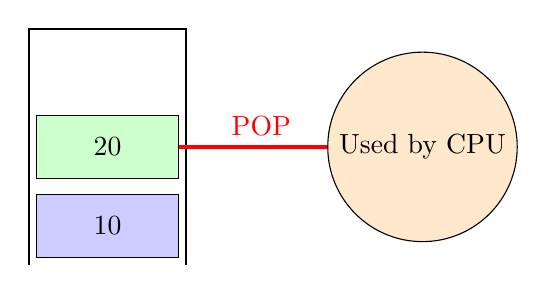
\begin{tikzpicture}
			% Stack
			\draw[thick] (0,0) -- (0,3) -- (2,3) -- (2,0);
			\node[draw, fill=blue!20, minimum width=1.8cm, minimum height=0.8cm] at (1, 0.5) {10};
			\node[draw, fill=green!20, minimum width=1.8cm, minimum height=0.8cm] (top) at (1, 1.5) {20};
			
			% Outgoing
			\draw[->, ultra thick, red] (top) -- (4, 1.5) node[midway, above] {POP};
			\node[draw, circle, fill=TechOrange!20] at (5, 1.5) {Used by CPU};
		\end{tikzpicture}
	\end{frame}
	
	% Slide 10: Operation EXECUTE (The Result)
	% FIXED: Requires shapes.symbols library
	\begin{frame}{Core Operation 3: EXECUTE \& RESULT}
		\textbf{EXECUTE:} The CPU calculates the answer and \textbf{PUSHES} it back.
		\vspace{0.5cm}
		\centering
		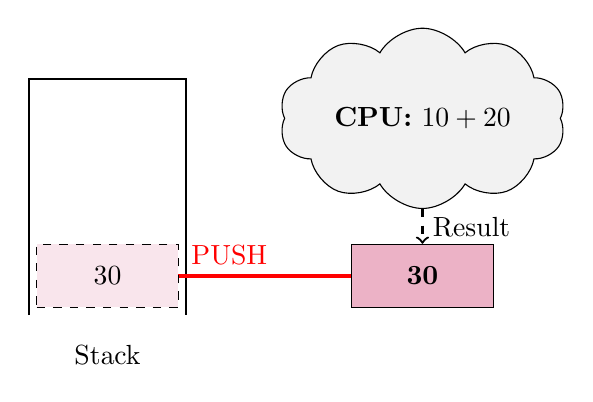
\begin{tikzpicture}
			% The Stack
			\draw[thick] (0,0) -- (0,3) -- (2,3) -- (2,0);
			\node at (1, -0.5) {Stack};
			
			% The Calculation (Cloud Shape)
			\node[cloud, draw, cloud puffs=10, cloud puff arc=120, aspect=2, fill=gray!10] (cpu) at (5, 2.5) {\textbf{CPU:} $10 + 20$};
			
			% The Result
			\node[draw, fill=purple!30, minimum width=1.8cm, minimum height=0.8cm] (result) at (5, 0.5) {\textbf{30}};
			
			% Arrows
			\draw[->, thick, dashed] (cpu) -- node[right] {Result} (result);
			\draw[->, ultra thick, red] (result) -- (1, 0.5) node[midway, above] {PUSH};
			
			% Ghosted Result
			\node[draw, dashed, fill=purple!10, minimum width=1.8cm, minimum height=0.8cm] at (1, 0.5) {30};
		\end{tikzpicture}
	\end{frame}
	
	% Slide 11: Advanced Ops - SWAP
	\begin{frame}{Advanced Operation: SWAP}
		\textbf{SWAP:} Exchanges the top two items. Critical for non-commutative math ($a - b$).
		\vspace{0.5cm}
		\centering
		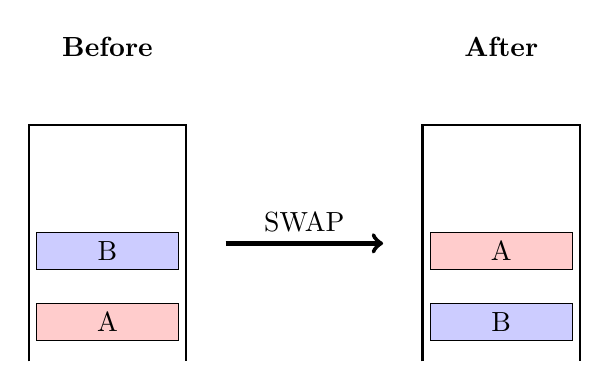
\begin{tikzpicture}
			% Before
			\node at (1, 4) {\textbf{Before}};
			\draw[thick] (0,0) -- (0,3) -- (2,3) -- (2,0);
			\node[draw, fill=red!20, minimum width=1.8cm] at (1, 0.5) {A};
			\node[draw, fill=blue!20, minimum width=1.8cm] at (1, 1.4) {B};
			
			% Arrow
			\draw[->, ultra thick] (2.5, 1.5) -- node[above]{SWAP} (4.5, 1.5);
			
			% After
			\node at (6, 4) {\textbf{After}};
			\draw[thick] (5,0) -- (5,3) -- (7,3) -- (7,0);
			\node[draw, fill=blue!20, minimum width=1.8cm] at (6, 0.5) {B};
			\node[draw, fill=red!20, minimum width=1.8cm] at (6, 1.4) {A};
		\end{tikzpicture}
	\end{frame}
	
	% Slide 12: Advanced Ops - ROT (Rotate)
	\begin{frame}{Advanced Operation: ROT (Rotate/Roll)}
		\textbf{ROT:} Cycles the top 3 items. The \textbf{3rd item} (Bottom) jumps to the Top.
		\vspace{0.2cm}
		\centering
		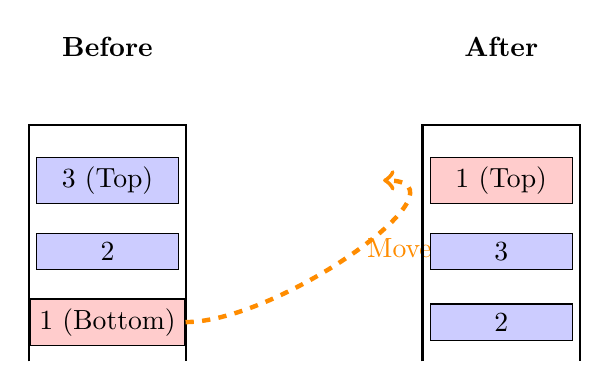
\begin{tikzpicture}
			% --- BEFORE STATE ---
			\node at (1, 4) {\textbf{Before}};
			\draw[thick] (0,0) -- (0,3) -- (2,3) -- (2,0);
			\node[draw, fill=red!20, minimum width=1.8cm] (item1) at (1, 0.5) {1 (Bottom)};
			\node[draw, fill=blue!20, minimum width=1.8cm] at (1, 1.4) {2};
			\node[draw, fill=blue!20, minimum width=1.8cm] at (1, 2.3) {3 (Top)};
			
			% --- ARROW ---
			\draw[->, ultra thick, dashed, TechOrange] (item1.east) to[out=0, in=0] node[right] {Moves to Top} (4.5, 2.3);
			
			% --- AFTER STATE ---
			\node at (6, 4) {\textbf{After}};
			\draw[thick] (5,0) -- (5,3) -- (7,3) -- (7,0);
			\node[draw, fill=blue!20, minimum width=1.8cm] at (6, 0.5) {2};
			\node[draw, fill=blue!20, minimum width=1.8cm] at (6, 1.4) {3};
			\node[draw, fill=red!20, minimum width=1.8cm] at (6, 2.3) {1 (Top)};
		\end{tikzpicture}
	\end{frame}
	
	% Slide 13: The Algorithm Rules
	\begin{frame}{The Algorithm Logic}
		\begin{enumerate}
			\item \textbf{Scan} input string from Left to Right.
			\item \textbf{If Number:} PUSH to stack.
			\item \textbf{If Operator:} 
			\begin{itemize}
				\item POP Top (B)
				\item POP Next (A)
				\item Calculate $A \ op \ B$
				\item PUSH Result
			\end{itemize}
		\end{enumerate}
	\end{frame}
	
	% ==========================================
	% PART 4: VISUAL TRACE (Slides 14-17)
	% ==========================================
	\section{Step-by-Step Trace}
	
	% Slide 14: Trace Start
	\begin{frame}{Visual Trace: $3 \quad 4 \quad +$}
		\textbf{Step 1:} Read "3". It is a number. \textbf{PUSH 3}.
		\vspace{1cm}
		\centering
		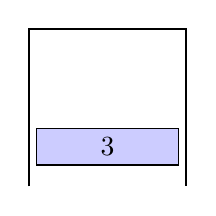
\begin{tikzpicture}
			\draw[thick] (0,0) -- (0,2) -- (2,2) -- (2,0);
			\node[draw, fill=blue!20, minimum width=1.8cm] at (1, 0.5) {3};
		\end{tikzpicture}
	\end{frame}
	
	% Slide 15: Trace Step 2
	\begin{frame}{Visual Trace: $3 \quad 4 \quad +$}
		\textbf{Step 2:} Read "4". It is a number. \textbf{PUSH 4}.
		\vspace{1cm}
		\centering
		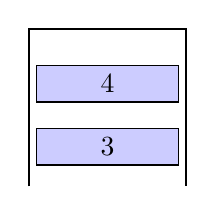
\begin{tikzpicture}
			\draw[thick] (0,0) -- (0,2) -- (2,2) -- (2,0);
			\node[draw, fill=blue!20, minimum width=1.8cm] at (1, 0.5) {3};
			\node[draw, fill=blue!20, minimum width=1.8cm] at (1, 1.3) {4};
		\end{tikzpicture}
	\end{frame}
	
	% Slide 16: Trace Step 3 (Calc)
	\begin{frame}{Visual Trace: $3 \quad 4 \quad +$}
		\textbf{Step 3:} Read "+". It is an operator.
		\begin{itemize}
			\item POP 4
			\item POP 3
			\item Calculate $3 + 4 = 7$
			\item \textbf{PUSH 7}
		\end{itemize}
		\vspace{0.5cm}
		\centering
		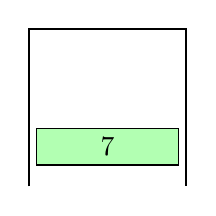
\begin{tikzpicture}
			\draw[thick] (0,0) -- (0,2) -- (2,2) -- (2,0);
			\node[draw, fill=green!30, minimum width=1.8cm] at (1, 0.5) {7};
		\end{tikzpicture}
	\end{frame}
	
	% Slide 17: Complex Example
	\begin{frame}{Complex Trace: $5 \quad 1 \quad 2 \quad + \quad 4 \quad \times \quad + \quad 3 \quad -$}
		Infix equivalent: $5 + ((1 + 2) \times 4) - 3$
		\vspace{0.5cm}
		\begin{table}
			\centering
			\small
			\begin{tabular}{l l l}
				\toprule
				\textbf{Input} & \textbf{Action} & \textbf{Stack} \\
				\midrule
				5 & Push 5 & [5] \\
				1 & Push 1 & [5, 1] \\
				2 & Push 2 & [5, 1, 2] \\
				+ & Pop 2, 1 $\rightarrow$ 3 & [5, 3] \\
				4 & Push 4 & [5, 3, 4] \\
				* & Pop 4, 3 $\rightarrow$ 12 & [5, 12] \\
				+ & Pop 12, 5 $\rightarrow$ 17 & [17] \\
				\dots & \dots & \dots \\
				\bottomrule
			\end{tabular}
		\end{table}
	\end{frame}
	
	% ==========================================
	% PART 5: IMPLEMENTATION (Slides 18-21)
	% ==========================================
	\section{Python Implementation}
	
	% Slide 18: Tech Stack
	\begin{frame}{Technology Stack}
		\begin{columns}
			\column{0.5\textwidth}
			\begin{block}{Backend}
				\begin{itemize}
					\item \textbf{Language:} Python 3.10
					\item \textbf{Logic:} List-based Stack
					\item \textbf{Math:} \texttt{operator} module
				\end{itemize}
			\end{block}
			
			\column{0.5\textwidth}
			\begin{block}{Frontend (GUI)}
				\begin{itemize}
					\item \textbf{Library:} Flet (Flutter for Python)
					\item \textbf{Features:} Keyboard support, Animations, Responsive Layout
				\end{itemize}
			\end{block}
		\end{columns}
	\end{frame}
	
	% Slide 19: Error Handling
	\begin{frame}{Handling Edge Cases}
		A robust calculator must handle errors gracefully.
		\vspace{0.5cm}
		\begin{enumerate}
			\item \textbf{Stack Underflow:} User presses "+" but stack only has 1 number.
			\item \textbf{Division by Zero:} User types `5 0 /`.
			\item \textbf{Invalid Input:} User types text instead of numbers.
		\end{enumerate}
		\vspace{0.5cm}
		\textbf{Solution:} We wrap execution in `try-except` blocks to prevent crashes.
	\end{frame}
	

	
	% Slide 21: LIVE DEMO
	\begin{frame}
		\centering
		\vspace{1cm}
		
\begin{tikzpicture}
			\node[draw, ultra thick, rounded corners, fill=TechOrange, text=white, drop shadow] 
			{\Huge \textbf{LIVE DEMO}};
		\end{tikzpicture}
		\vspace{1cm}
		
		\Large \textit{Switching to Application...}
	\end{frame}
	
	% ==========================================
	% PART 6: CONCLUSION (Slides 22-25)
	% ==========================================
	\section{Conclusion}
	
	% Slide 22: Pros of RPN (FIXED MATH MODE)
	\begin{frame}{Advantages of Reverse Polish Notation (RPN)}
		Why do engineers prefer this system?
		\vspace{0.3cm}
		\begin{itemize}
			\item[\textcolor{green}{$\checkmark$}] \textbf{Zero Parentheses:} You never need to type `(` or `)`. Order is defined by stack.
			\item[\textcolor{green}{$\checkmark$}] \textbf{Keystroke Efficiency:} Studies show RPN requires fewer button presses.
			\item[\textcolor{green}{$\checkmark$}] \textbf{Computer Native:} It aligns perfectly with how CPUs process logic.
			\item[\textcolor{green}{$\checkmark$}] \textbf{Intermediate Results:} You see the answer to every step.
		\end{itemize}
	\end{frame}
	
	% Slide 23: Cons of RPN (FIXED MATH MODE)
	\begin{frame}{Disadvantages \& Challenges}
		Why isn't everyone using it?
		\vspace{0.3cm}
		\begin{itemize}
			\item[\textcolor{red}{$\times$}] \textbf{Steep Learning Curve:} It feels "backwards" to anyone taught school math ($3+4$).
			\item[\textcolor{red}{$\times$}] \textbf{Readability:} `3 4 5 * +` is hard to read on paper vs $3 + (4 \times 5)$.
			\item[\textcolor{red}{$\times$}] \textbf{Mental Load:} You must keep track of the "Stack Depth" to avoid errors.
		\end{itemize}
	\end{frame}
	
	% Slide 24: Summary
	\begin{frame}{Project Summary}
		\begin{itemize}
			\item We explored the history of \textbf{HP Calculators}.
			\item We mastered the \textbf{Stack Data Structure}.
			\item We built a fully functional \textbf{Python GUI}.
			\item We implemented advanced operations like \textbf{SWAP} and \textbf{ROT}.
		\end{itemize}
	\end{frame}
	
	% Slide 25: Thank You
	\begin{frame}
		\centering
		\vspace{1.5cm}
		\Huge \textbf{Thank You!}
		
		\vspace{1cm}
		\normalsize
		\textbf{Questions?}
	\end{frame}
	
\end{document}